\chapter{Creación del certificado del servidor www.ejemplo.com y ejemplo.com}
En este apartado se detalla la creación del certificado de servidor firmado con 
la autoridad de la asignatura, asegurándose de que el certificado incorpora 
correctamente dichos nombres en la extensión \texttt{subjectAltName}.
\section{Enunciado}
1. Creación del certificado del servidor \texttt{www.ejemplo.com} (y \texttt{ejemplo.com}) firmado con la autoridad de la asignatura. Asegurarse de que el certificado incorpora correctamente los nombres \texttt{www.ejemplo.com} y \texttt{ejemplo.com} en la extensión \texttt{subjectAltName}.
\section{Resolución}
Para incluir las extensiones requeridas se crea un fichero \texttt{extensiones\_v3.cnf} 
con el siguiente contenido:
\begin{lstlisting}[language=bash]
#### EXTENSIONES PARA subjectAltName
[ v3_req ]
# Extensions to add a certificate request
subjectAltName = @alt_names
basicConstraints = CA:FALSE
keyUsage = nonRepudiation, digitalSignature, keyEncipherment
[alt_names]
DNS.1 = www.ejemplo.com
DNS.2 = ejemplo.com
\end{lstlisting}

La orden de generación con OpenSSL será la siguiente:
\begin{lstlisting}[language=bash]
    openssl req -new \
-subj "/C=ES/ST=LasPalmas/O=Ejemplo/CN=www.ejemplo.com"
-subj=C=ES/ST=LasPalmas/O=Ejemplo/CN="www.ejemplo.com"
-in servidor.csr
-subj=/C=ES/ST=LasPalmas/O=Ejemplo/CN=www.ejemplo.com
-key servidor.key
-out servidor.csr
-subj="/C=ES/ST=LasPalmas/O=Ejemplo/CN=www.ejemplo.com"
-extfile ext_v3.cnf
-extensions v3_req
\end{lstlisting}
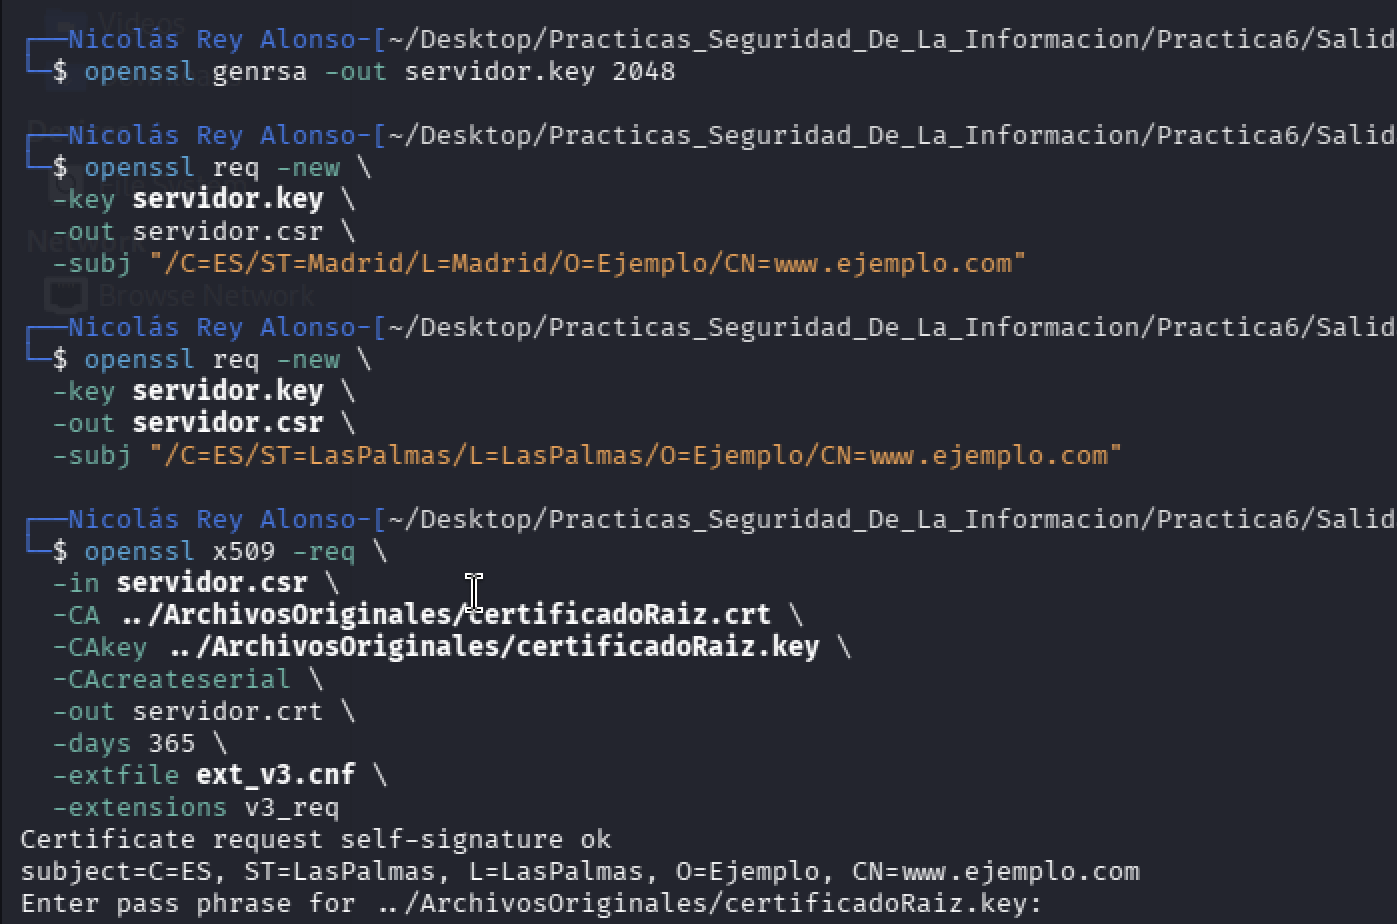
\includegraphics[width=0.8\textwidth]{Imagenes/4.png}

